\documentclass[final]{beamer}
%% Possible paper sizes: a0, a0b, a1, a2, a3, a4.
%% Possible orientations: portrait, landscape
%% Font sizes can be changed using the scale option.
\usepackage[size=a0,orientation=portrait,scale=1.2]{beamerposter}
\usepackage[backend=biber,style=numeric,sorting=none]{biblatex}
\usepackage[version=4]{mhchem}

\addbibresource{biblio_poster.bib}

\definecolor{cadmiumgreen}{rgb}{0.0, 0.42, 0.24}
\definecolor{asparagus}{rgb}{0.53, 0.66, 0.42}

\newcommand{\red}[1]{\textcolor{red}{#1}}
\newcommand{\blue}[1]{\textcolor{blue}{#1}}
\newcommand{\green}[1]{\textcolor{green}{#1}}
\newcommand{\purple}[1]{\textcolor{purple}{#1}}
\newcommand{\cadmiumgreen}[1]{\textcolor{cadmiumgreen}{#1}}
\newcommand{\asparagus}[1]{\textcolor{asparagus}{#1}}

\AtEveryBibitem{%
\ifentrytype{article}{
    \clearfield{url}%
    \clearfield{urlyear}%
    \clearfield{doi}%
    \clearfield{issn}%
    \clearfield{month}%
    \clearfield{day}%
    \clearfield{title}%
}{}
}

\DeclareFieldFormat[article]{pages}{#1}

\renewbibmacro{in:}{%
  \ifentrytype{article}{}{\printtext{\bibstring{in}\intitlepunct}}}

\usetheme{gemini}
%\usecolortheme{gemini}
\usecolortheme{geminigreen}
\useinnertheme{rectangles}

% ====================
% Packages
% ====================

\usepackage[utf8]{inputenc}
\usepackage{graphicx,dcolumn,xcolor,microtype,multirow,amscd,amsmath,amssymb,amsfonts,physics,wrapfig,tikz,siunitx,bm}
\usepackage{booktabs}
\usepackage{tikz}
\usepackage{pgfplots}

\newfontfamily\qp{Times New Roman}[
  % the font has no small caps, so we use another one for them
  SmallCapsFont=TeX Gyre Termes,
  SmallCapsFeatures={Letters=SmallCaps}
]


% ====================
% Lengths
% ====================

% If you have N columns, choose \sepwidth and \colwidth such that
% (N+1)*\sepwidth + N*\colwidth = \paperwidth
\newlength{\sepwidth}
\newlength{\colwidth}
\newlength{\threesepwidth}
\newlength{\threecolwidth}
\newlength{\foursepwidth}
\newlength{\fourcolwidth}
\setlength{\sepwidth}{0.03\paperwidth}
\setlength{\colwidth}{0.45\paperwidth}
\setlength{\threesepwidth}{0.03\paperwidth}
\setlength{\threecolwidth}{0.30\paperwidth}
\setlength{\foursepwidth}{0.03\paperwidth}
\setlength{\fourcolwidth}{0.22\paperwidth}

\newcommand{\separatorcolumn}{\begin{column}{\sepwidth}\end{column}}
\newcommand{\threeseparatorcolumn}{\begin{column}{\threesepwidth}\end{column}}
\newcommand{\fourseparatorcolumn}{\begin{column}{\foursepwidth}\end{column}}


% ====================
% Logo (optional)
% ====================

% LaTeX logo taken from https://commons.wikimedia.org/wiki/File:LaTeX_logo.svg
% use this to include logos on the left and/or right side of the header:
\logoright{\vspace{6cm} 
\includegraphics[width=8cm]{fig/Fermi.jpg}}
\logoleft{\vspace{-5cm} 
\includegraphics[width=8cm]{fig/ERC.jpg}}% \hspace{1cm} 
\includegraphics[height=6cm]{fig/CNRS.png} }
\addtobeamertemplate{headline}{} 
{
\begin{tikzpicture}[remember picture,overlay] 
\node [shift={(7.5 cm,-3.2cm)}] at (current page.north west) {
\includegraphics[height=5cm]{fig/CNRS.png}}; 
\node [shift={(-6.30 cm,-4cm)}] at (current page.north east) {
\includegraphics[width=8cm]{fig/LCPQ.jpg}}; 
\end{tikzpicture} 
}

% ====================
% Footer (optional)
% ====================

\footercontent{
	Hierarchy Configuration Interaction
	\hfill
	F\'abris Kossoski \textit{et al.} (LCPQ)
	\hfill
	\href{mailto:fkossoski@irsamc.ups-tlse.fr}{\texttt{fkossoski@irsamc.ups-tlse.fr}}
}
% (can be left out to remove footer)

% ====================
% My own customization
% - BibLaTeX
% - Boxes with tcolorbox
% - User-defined commands
% ====================
%\input{custom-defs.tex}

%% Reference Sources
%\addbibresource{refs.bib}
%\renewcommand{\pgfuseimage}[1]{\includegraphics[scale=2.0]{#1}}

\newcommand{\LCPQ}{Laboratoire de Chimie et Physique Quantiques (UMR 5626), Universit\'e de Toulouse, CNRS, UPS, France}

\title{Unifying excitation degree and seniority number into a single hierarchy parameter}

%\author{F\'abris Kossoski,\inst{1} Yann Damour,\inst{1} and Pierre-Fran\c{c}ois Loos\inst{1}}
%\institute[shortinst]{\inst{1} \LCPQ}
\author{\underline{F\'abris Kossoski}, Yann Damour, and Pierre-Fran\c{c}ois Loos}
\institute[shortinst]{\LCPQ}

\begin{document}

\begin{frame}[t]

%%%%%%%%%%%%%%%%%%%%%%%%%%%%%%%%%%%%%%%%%%%%%%%%%%%%%%%%%%%%%%%%%%%%%%%%%%%%%%%%%%%%%%%%%%%%%%%%%%%%%%%%%%%%%%%%%%%%%%%%%%%%%%%%%%%%%%%%%%%%%%%%%%
\begin{alertblock}{Abstract}
Starting from a reference determinant, including excitations of progressively larger degree (singles, doubles, etc.) represent a very natural way to move towards the exact full configuration interaction (CI) limit. Over the past few years, an alternative pathway that connects the mean-field and the exact solution has been explored, based on the concept of seniority (number of unpaired electrons in a given determinant). While excitation-based CI performs well at weak correlation regimes, it struggles at strong correlation regimes, where seniority-based CI excels. Unfortunately, the computational cost of the latter class of CI scales exponentially with the number of basis functions, whereas the former one scales only polynomially. Given this background, here we present a new way of partitioning the Hilbert space, based on a hierarchy parameter that combines both the seniority number and the excitation degree. The new method, labelled hierarchy CI (hCI), is compared with its excitation-based and seniority-based counterparts, as well as with numerically exact results, for several challenging chemical systems and different properties. We found that hCI inherits desirable properties from both its parents. In particular, hCI provides a more balanced description of weak and strong correlation, at a polynomial cost. We further discuss the impact of optimizing the orbitals for the three different classes of CI.
\end{alertblock}
%%%%%%%%%%%%%%%%%%%%%%%%%%%%%%%%%%%%%%%%%%%%%%%%%%%%%%%%%%%%%%%%%%%%%%%%%%%%%%%%%%%%%%%%%%%%%%%%%%%%%%%%%%%%%%%%%%%%%%%%%%%%%%%%%%%%%%%%%%%%%%%%%%

\begin{columns}[t]
\separatorcolumn

\begin{column}{\colwidth}

%%%%%%%%%%%%%%%%%%%%%%%%%%%%%%%%%%%%%%%%%%%%%%%%%%%%%%%%%%%%%%%%%%%%%%%%%%%%%%%%%%%%%%%%%%%%%%%%%%%%%%%%%%%%%%%%%%%%%%%%%%%%%%%%%%%%%%%%%%%%%%%%%%
\vspace{-1.5cm}
\begin{block}{Different flavours of configuration interaction (CI)}

We present {\bf hierarchy configuration interaction (hCI)} \cite{Kossoski_2022}, defined by 
\begin{equation*}
  \boxed{\green{h} = \frac{\red{e} + \blue{s}/2}{2}}
\end{equation*}
\vspace{-1.5cm}
\begin{itemize}
    \item \green{$h$: hierarchy parameter}
    \item \red{$e$: excitation degree} (with respect to a closed-shell determinant)
    \item \blue{$s$: seniority number} (number of unpaired electrons of a determinant)
\end{itemize}

Implemented in the open-source software {\qp{QUANTUM PACKAGE}} \cite{Garniron_2019} \\ \url{https://quantumpackage.github.io/qp2/}.
\begin{figure}
  \centering
  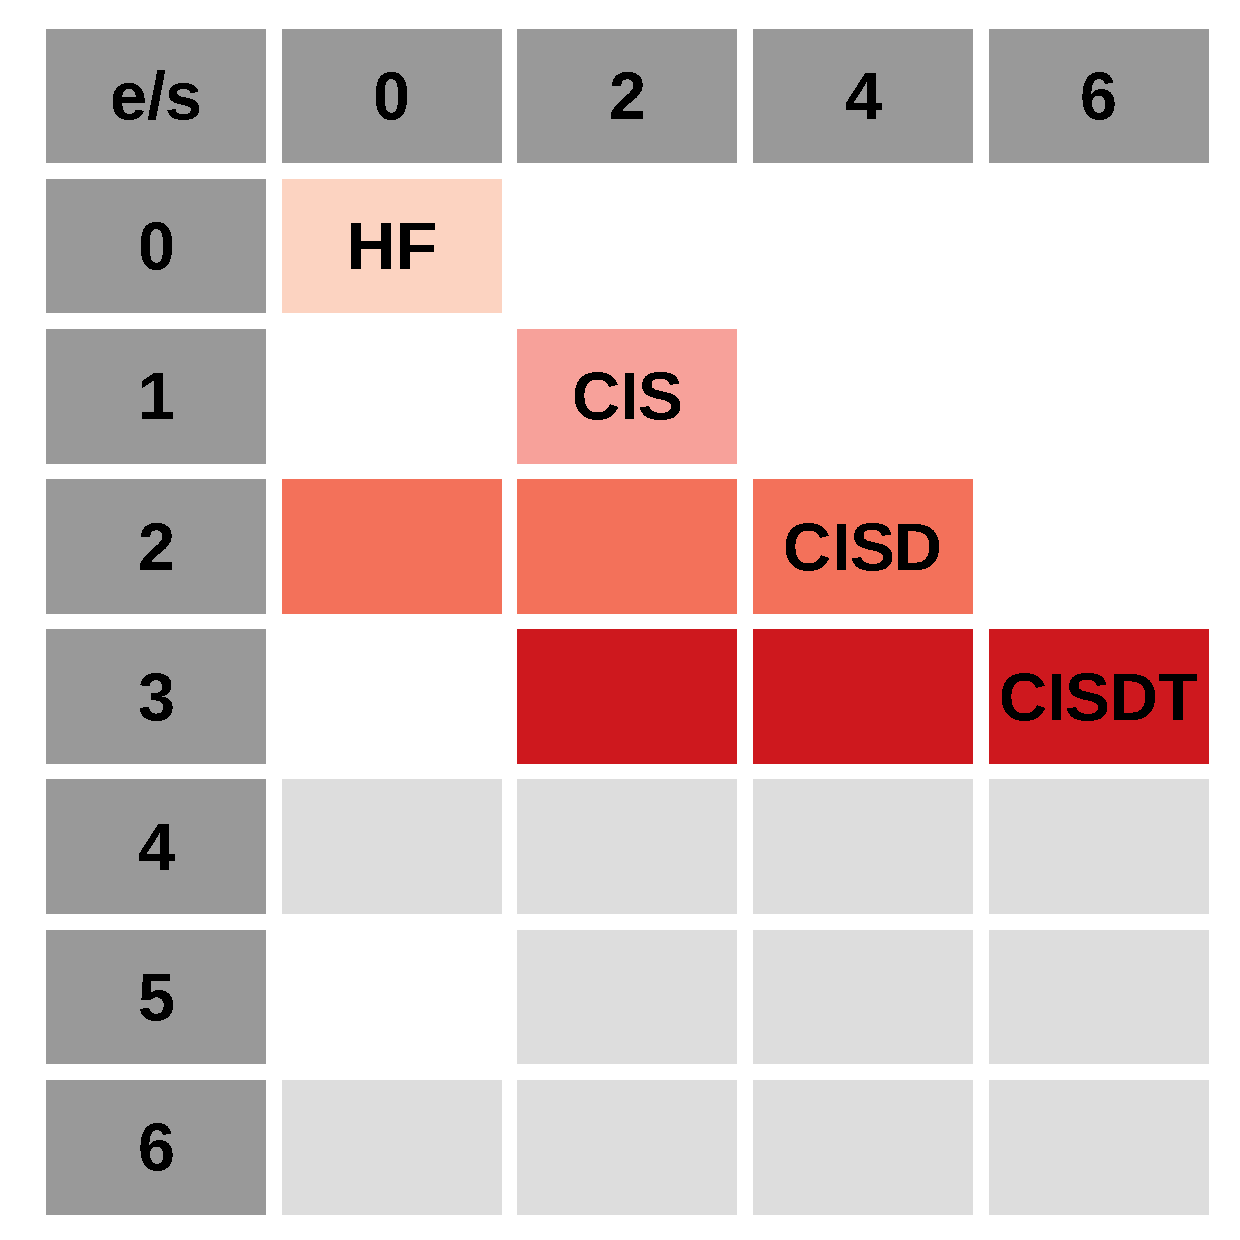
\includegraphics[width=0.32\textwidth]{fig/table_exc_full.pdf}
  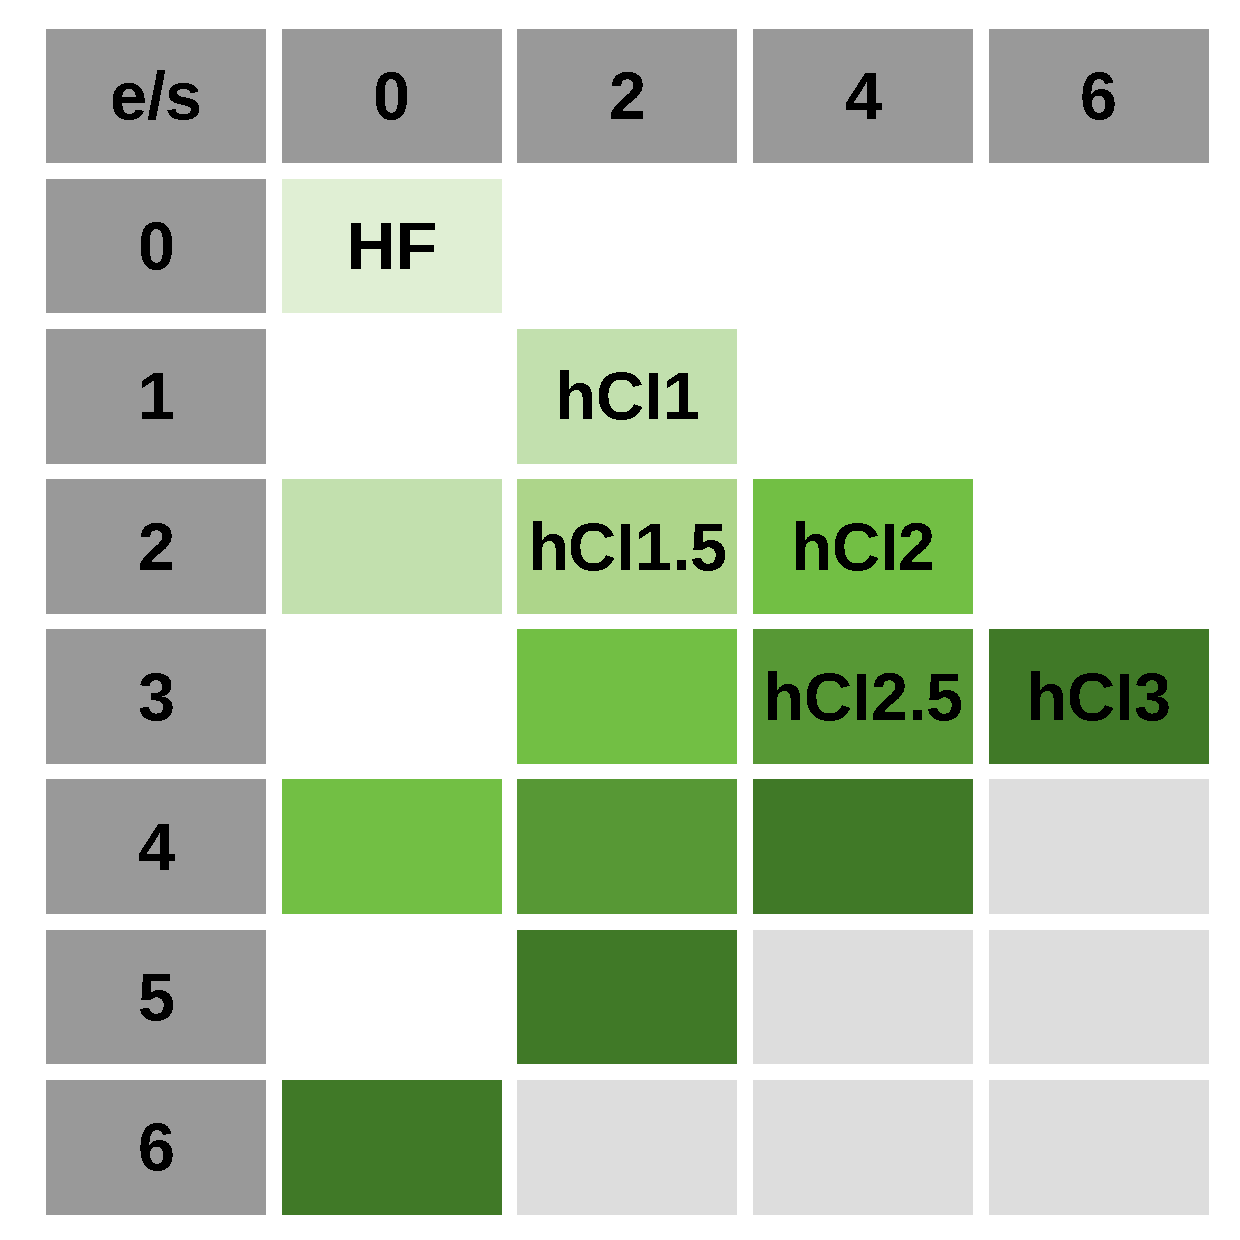
\includegraphics[width=0.32\textwidth]{fig/table_hCI.pdf}
  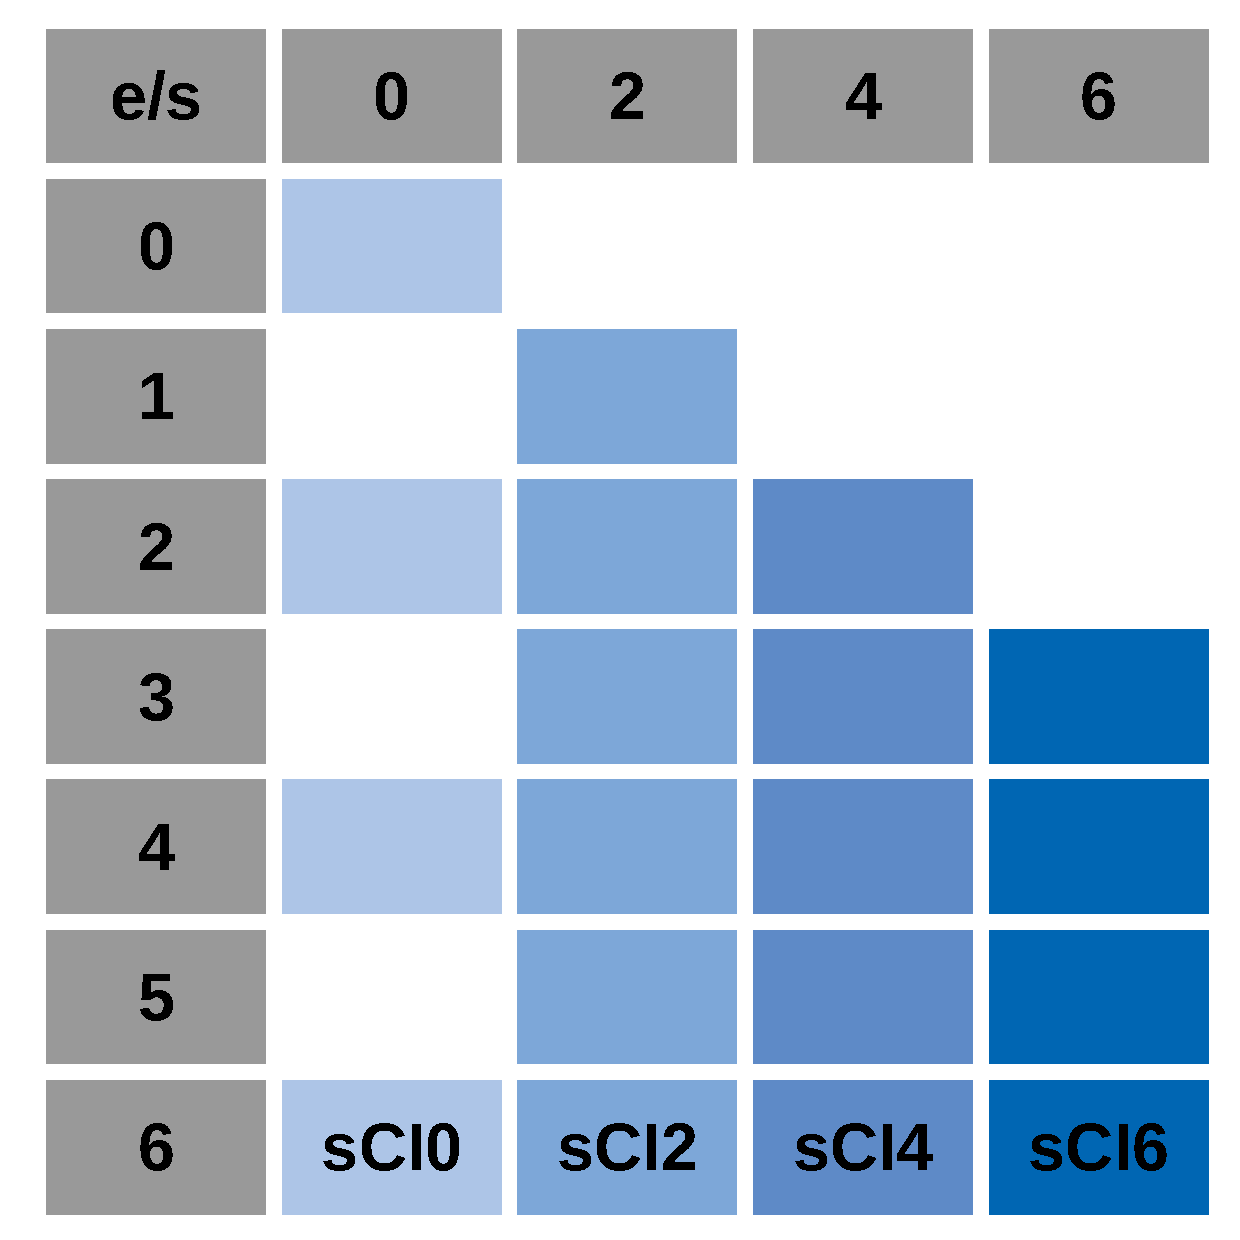
\includegraphics[width=0.32\textwidth]{fig/table_sen_full.pdf}
  \caption{$e$-$s$ map of the Hilbert space, truncated differently in excitation-based CI (eCI), left, seniority-based CI (sCI), right, and hierarchy-based CI (hCI), center. The color tones represent the determinants that are included at a given CI level.}
  \label{fig:table_exc}
\end{figure}
\vspace{-0.5cm}
{\bf What motivates this new flavour of CI?}
\vspace{-0.5cm}
\begin{itemize}
  \item {\bf Physics}: we aim at recovering both static correlation (well described by sCI) as well as dynamic correlation (where eCI performs well)
  \item {\bf Computational}: the number of determinants in a given diagonal has the same (polynomial) scaling with system size
  \item {\bf Empirical}: Any partitioning is possible, is this one effective?
\end{itemize}
\end{block}
%%%%%%%%%%%%%%%%%%%%%%%%%%%%%%%%%%%%%%%%%%%%%%%%%%%%%%%%%%%%%%%%%%%%%%%%%%%%%%%%%%%%%%%%%%%%%%%%%%%%%%%%%%%%%%%%%%%%%%%%%%%%%%%%%%%%%%%%%%%%%%%%%%


%%%%%%%%%%%%%%%%%%%%%%%%%%%%%%%%%%%%%%%%%%%%%%%%%%%%%%%%%%%%%%%%%%%%%%%%%%%%%%%%%%%%%%%%%%%%%%%%%%%%%%%%%%%%%%%%%%%%%%%%%%%%%%%%%%%%%%%%%%%%%%%%%%
\begin{block}{Typical example: dissociation of \ce{N2}}
  \vspace{-0.5cm}
  \begin{figure}
    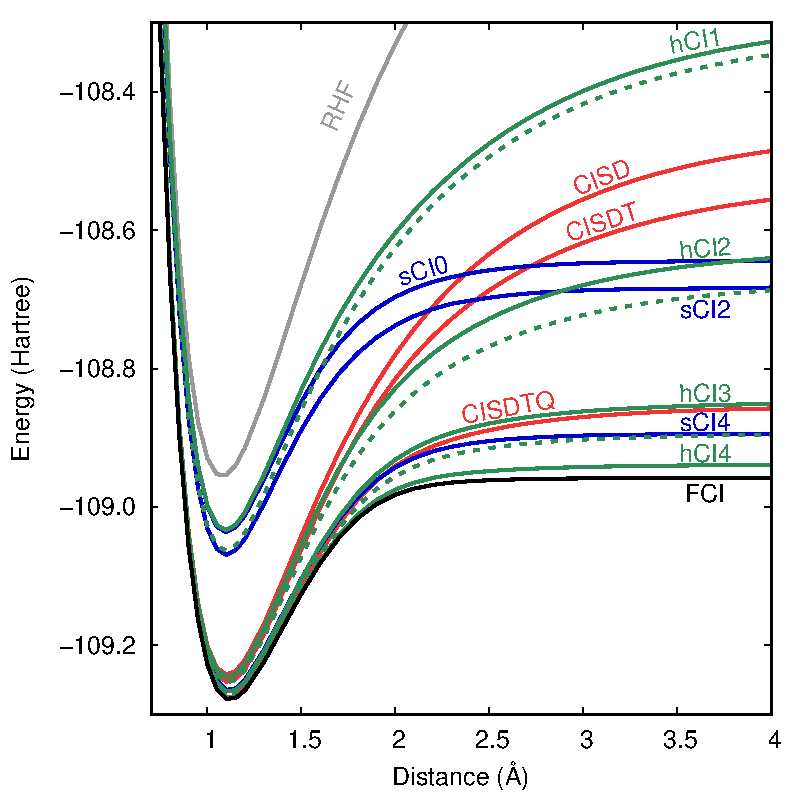
\includegraphics[width=0.67\textwidth]{fig/plot_pes_3.pdf}
    \caption{Potential energy curves for \ce{N2}, according to RHF, FCI, sCI (blue), eCI (red), and hCI (green) (dashed lines for half-integer $h$), with HF orbitals, and with the cc-pVDZ basis set.}
    \label{fig:plot_pes_3}
  \end{figure}
\end{block}
%%%%%%%%%%%%%%%%%%%%%%%%%%%%%%%%%%%%%%%%%%%%%%%%%%%%%%%%%%%%%%%%%%%%%%%%%%%%%%%%%%%%%%%%%%%%%%%%%%%%%%%%%%%%%%%%%%%%%%%%%%%%%%%%%%%%%%%%%%%%%%%%%%

%%%%%%%%%%%%%%%%%%%%%%%%%%%%%%%%%%%%%%%%%%%%%%%%%%%%%%%%%%%%%%%%%%%%%%%%%%%%%%%%%%%%%%%%%%%%%%%%%%%%%%%%%%%%%%%%%%%%%%%%%%%%%%%%%%%%%%%%%%%%%%%%%%
\vspace{-1.5cm}
\begin{block}{References}
  \vspace{-0.5cm}
  \printbibliography
\end{block}
%%%%%%%%%%%%%%%%%%%%%%%%%%%%%%%%%%%%%%%%%%%%%%%%%%%%%%%%%%%%%%%%%%%%%%%%%%%%%%%%%%%%%%%%%%%%%%%%%%%%%%%%%%%%%%%%%%%%%%%%%%%%%%%%%%%%%%%%%%%%%%%%%%

\end{column}


\begin{column}{\colwidth}

%%%%%%%%%%%%%%%%%%%%%%%%%%%%%%%%%%%%%%%%%%%%%%%%%%%%%%%%%%%%%%%%%%%%%%%%%%%%%%%%%%%%%%%%%%%%%%%%%%%%%%%%%%%%%%%%%%%%%%%%%%%%%%%%%%%%%%%%%%%%%%%%%%
\vspace{-1.5cm}
\begin{block}{Nonparallelity errors and vibrational frequencies}
  \vspace{-0.5cm}
  \begin{figure}
    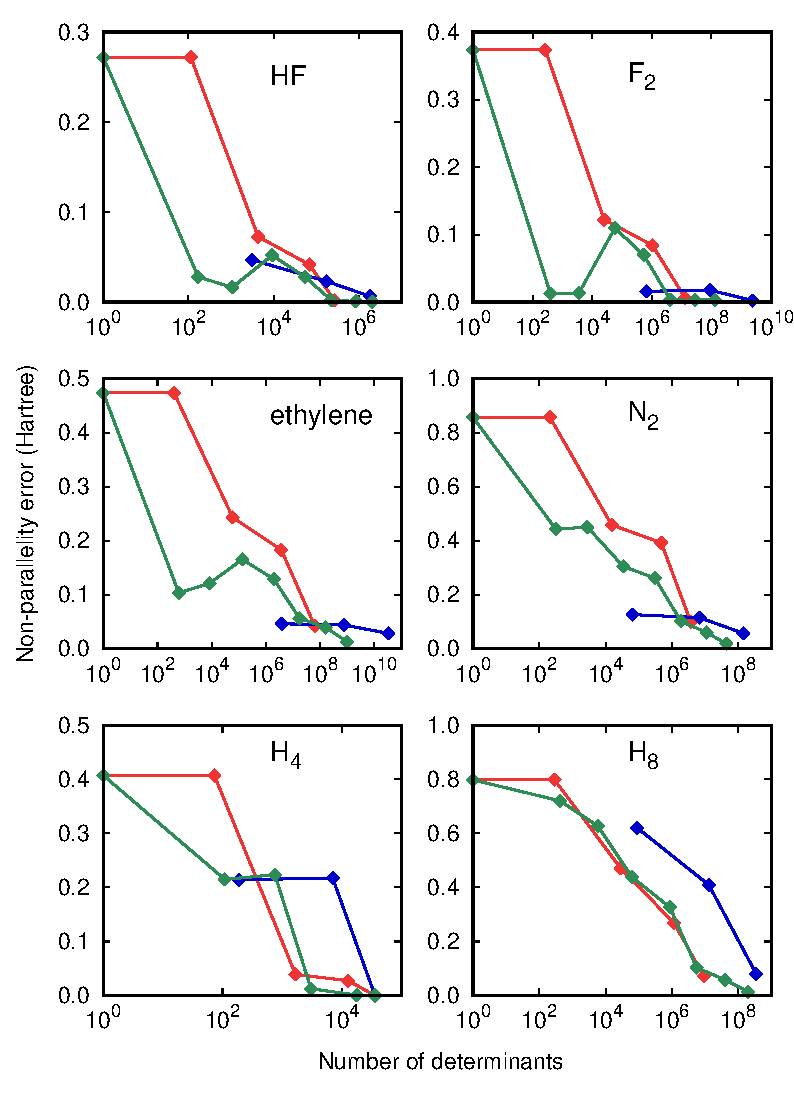
\includegraphics[width=0.47\textwidth]{fig/plot_stat.pdf}
    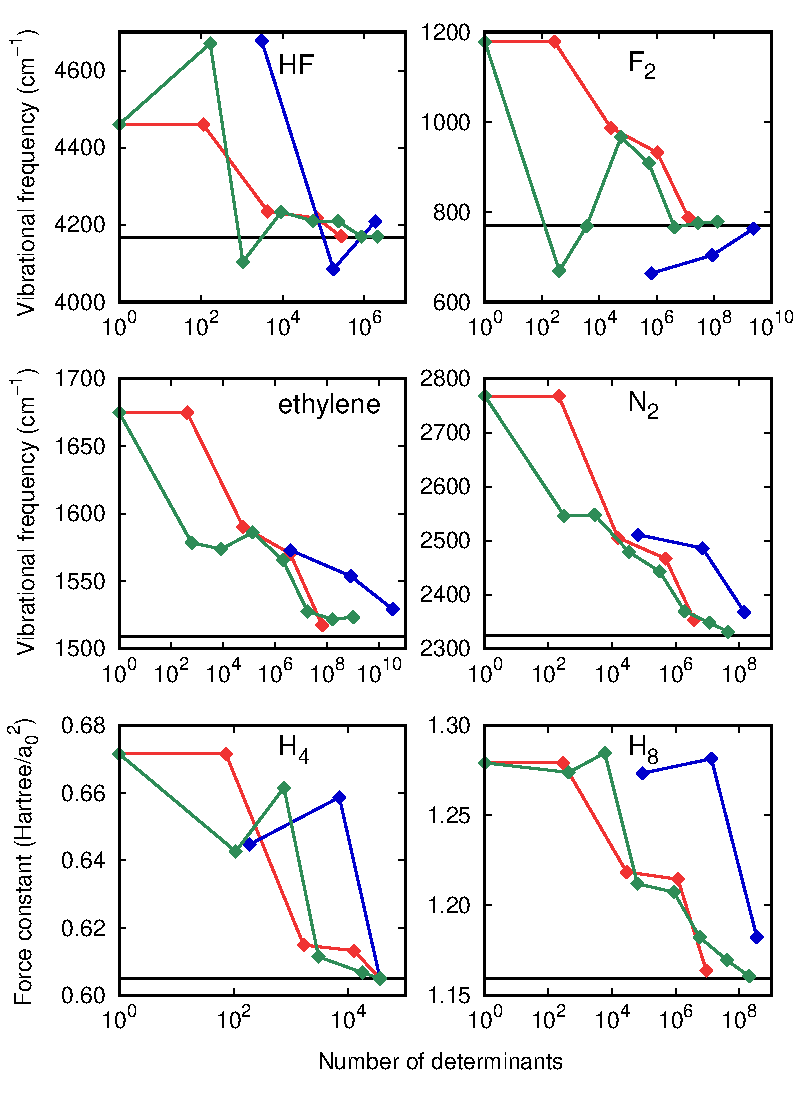
\includegraphics[width=0.47\textwidth]{fig/freq.pdf}
    \caption{Nonparallelity errors (left) and vibrational frequencies (right) as a function of the number of determinants, for sCI (blue), eCI (red), and hCI (green).}
    \label{fig:plot_stat_distance}
  \end{figure}
\end{block}
%%%%%%%%%%%%%%%%%%%%%%%%%%%%%%%%%%%%%%%%%%%%%%%%%%%%%%%%%%%%%%%%%%%%%%%%%%%%%%%%%%%%%%%%%%%%%%%%%%%%%%%%%%%%%%%%%%%%%%%%%%%%%%%%%%%%%%%%%%%%%%%%%%

%%%%%%%%%%%%%%%%%%%%%%%%%%%%%%%%%%%%%%%%%%%%%%%%%%%%%%%%%%%%%%%%%%%%%%%%%%%%%%%%%%%%%%%%%%%%%%%%%%%%%%%%%%%%%%%%%%%%%%%%%%%%%%%%%%%%%%%%%%%%%%%%%%
\vspace{-1.5cm}
\begin{block}{Orbital optimized configuration interaction (oo-CI)}
  \vspace{-0.5cm}
  \begin{figure}
    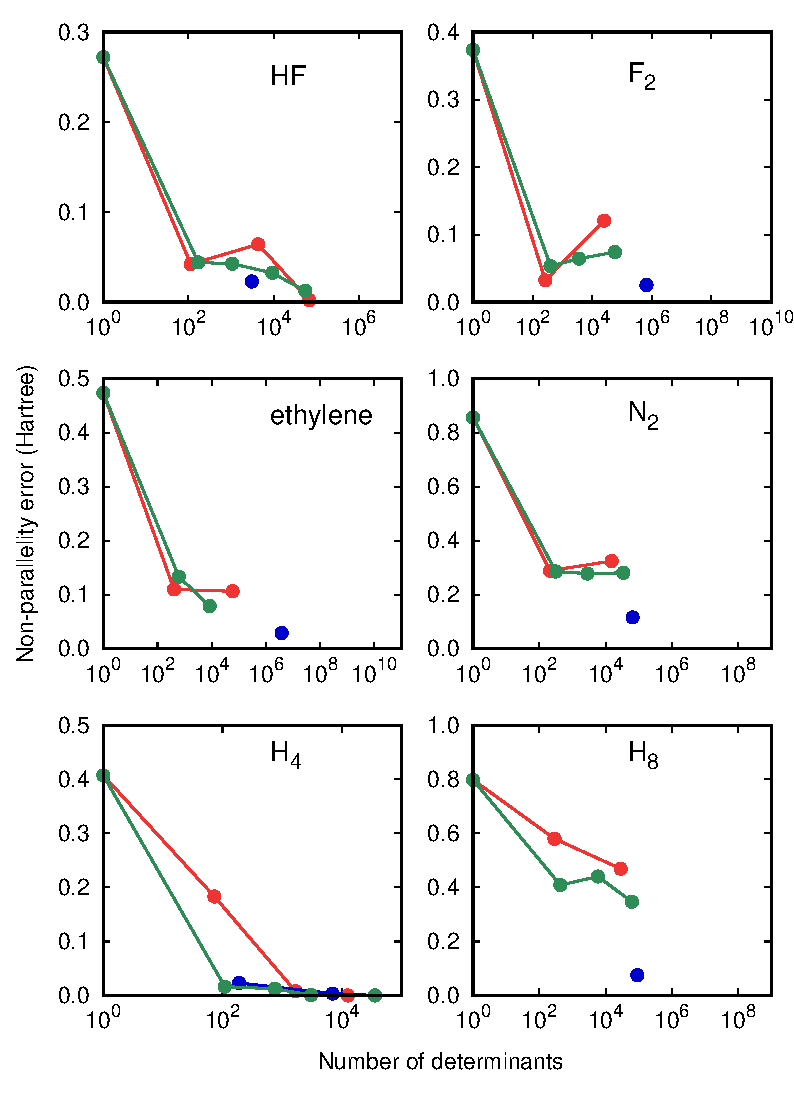
\includegraphics[width=0.47\textwidth]{fig/plot_stat_opt.pdf}
    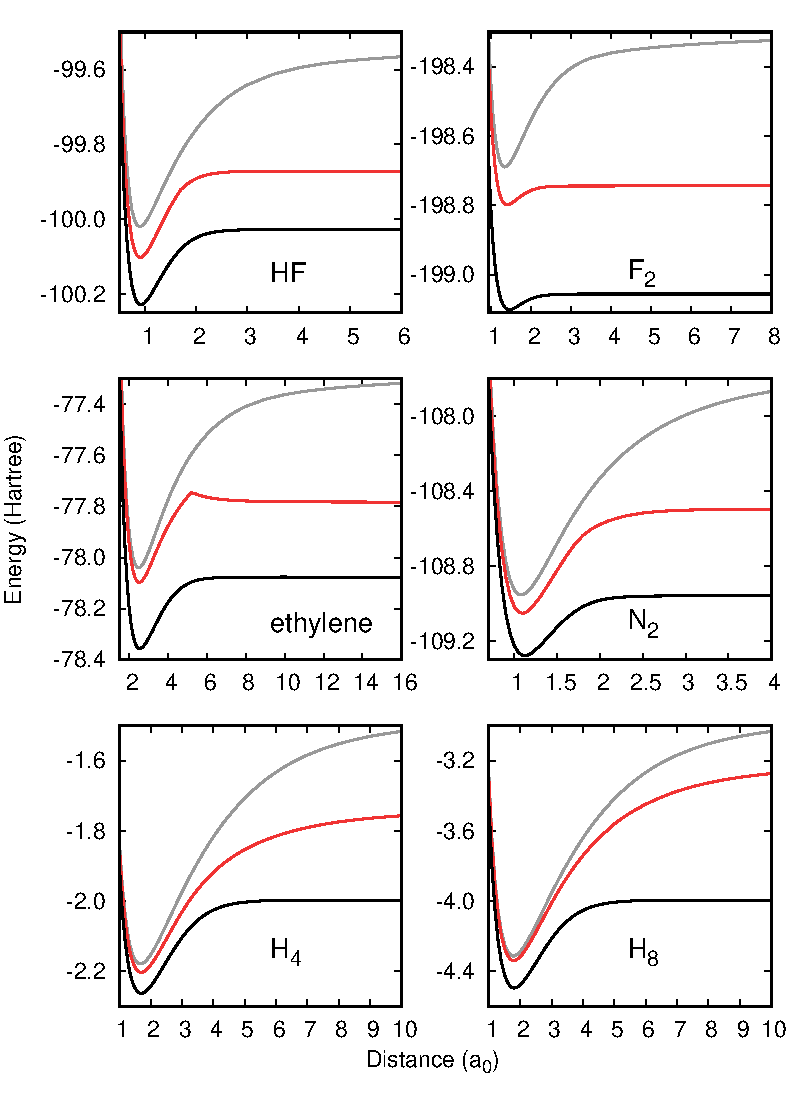
\includegraphics[width=0.47\textwidth]{fig/plot_pes_ooCIS.pdf}
    \caption{Left: nonparallelity errors as function of the number of determinants, for sCI (blue), eCI (red), and hCI (green), with orbitals optimized at each CI level \cite{Damour_2021}.
Right: potential energy curves according to RHF (gray), oo-CIS (red), and FCI (black).}
    \label{fig:plot_ooCI}
  \end{figure}
\end{block}
%%%%%%%%%%%%%%%%%%%%%%%%%%%%%%%%%%%%%%%%%%%%%%%%%%%%%%%%%%%%%%%%%%%%%%%%%%%%%%%%%%%%%%%%%%%%%%%%%%%%%%%%%%%%%%%%%%%%%%%%%%%%%%%%%%%%%%%%%%%%%%%%%%

%%%%%%%%%%%%%%%%%%%%%%%%%%%%%%%%%%%%%%%%%%%%%%%%%%%%%%%%%%%%%%%%%%%%%%%%%%%%%%%%%%%%%%%%%%%%%%%%%%%%%%%%%%%%%%%%%%%%%%%%%%%%%%%%%%%%%%%%%%%%%%%%%%
\vspace{-1.5cm}
\begin{block}{Summary}
  \vspace{-0.5cm}
  \begin{itemize}
    \item {\bf hCI}: Novel CI route, physically, computationally, and empirically inspired
    \item {\bf Performance}: overall superior than excitation-based CI, for different systems, properties, and basis sets
    \item {\bf Orbital optimization}: not always recommended, stepping up the CI ladder might be a wiser choice
    \item {\bf oo-CIS}: minimally correlated model (only single excitations), promising results
  \end{itemize}
\end{block}
%%%%%%%%%%%%%%%%%%%%%%%%%%%%%%%%%%%%%%%%%%%%%%%%%%%%%%%%%%%%%%%%%%%%%%%%%%%%%%%%%%%%%%%%%%%%%%%%%%%%%%%%%%%%%%%%%%%%%%%%%%%%%%%%%%%%%%%%%%%%%%%%%%

%%%%%%%%%%%%%%%%%%%%%%%%%%%%%%%%%%%%%%%%%%%%%%%%%%%%%%%%%%%%%%%%%%%%%%%%%%%%%%%%%%%%%%%%%%%%%%%%%%%%%%%%%%%%%%%%%%%%%%%%%%%%%%%%%%%%%%%%%%%%%%%%%%
\vspace{-1.5cm}
\begin{block}{Perspectives}
  \vspace{-0.5cm}
  \begin{itemize}
    \item {\bf hCI}: excited-states, open-shell systems, trial wave functions for quantum Monte Carlo, hierarchy coupled cluster
    \item {\bf Orbital optimization}: optimize at a lower level of CI, then run a higher level
    \item {\bf oo-CIS}: excited states
  \end{itemize}
\end{block}
%%%%%%%%%%%%%%%%%%%%%%%%%%%%%%%%%%%%%%%%%%%%%%%%%%%%%%%%%%%%%%%%%%%%%%%%%%%%%%%%%%%%%%%%%%%%%%%%%%%%%%%%%%%%%%%%%%%%%%%%%%%%%%%%%%%%%%%%%%%%%%%%%%

\end{column}

\separatorcolumn
\end{columns}

%%%%%%%%%%%%%%%%%%%%%%%%%%%%%%%%%%%%%%%%%%%%%%%%%%%%%%%%%%%%%%%%%%%%%%%%%%%%%%%%%%%%%%%%%%%%%%%%%%%%%%%%%%%%%%%%%%%%%%%%%%%%%%%%%%%%%%%%%%%%%%%%%%
\vspace{-1.5cm}
\begin{block}{Acknowledgement}
  \centering
  \textit{This project has received funding from the European Research Council (ERC) under the European Union's Horizon 2020 research and innovation programme, grant agreement No.~863481.}
\end{block}
%%%%%%%%%%%%%%%%%%%%%%%%%%%%%%%%%%%%%%%%%%%%%%%%%%%%%%%%%%%%%%%%%%%%%%%%%%%%%%%%%%%%%%%%%%%%%%%%%%%%%%%%%%%%%%%%%%%%%%%%%%%%%%%%%%%%%%%%%%%%%%%%%%

\end{frame}

\end{document}
